\chapter{Evaluation and Comparisons}
\label{chapter:Evaluation_and_Comparisons}

We have described the implementation of a push-pull signal-function FRP system.
Push-based event evaluation should have advantages in event latency and overall
performance over pull-based event evaluation. We would also like to compare
the evaluation interface in the current widely-used system with the one proposed
here, again in order to verify that the theoretical benefits do appear in
practice.

One way to evaluate this is to write an application in two systems, and benchmark
these systems for comparison. In order to compare TimeFlies with Yampa, the most
recently released pull-based signal-function FRP system, we decided to implement
a suitable application in both.

\section{Evaluation Application}
\label{section:Evaluation_and_Comparisons-Evaluation_Application}

The application of choice is a learning switch controller for OpenFlow~\cite{OpenflowSpec}
switches. This application must handle input events triggered by switches
signalling that they have received a packet for which they have no handling
rules, and produce output events which install handling rules for dealing with
these packets.

The reactive algorithm is simple. A table from machine addresses to switch ports
is maintained. This table is updated in two ways. When a packet is sent to the
controller, meta-data for the packet indicates which port it arrived on. The
source address of the packet can then be mapped to that port in the table.
Once this occurs, rules are installed for each packet with a destination address
matching the source, along with reciprocal rules.

Each mapping in the table has a timestamp. After a certain amount of time, the
table entry is deleted. The table entry is also deleted if a packet is received
with the same source address and a different port. When an entry is deleted,
the switch is signaled to remove all corresponding rules.

In both Yampa and TimeFlies, this algorithm is implemented by using an accumulator,
which applies functions carried by event occurrences to a state value. It stores
the new state and outputs new event occurrences based on the output of the function.

The state stored is the table (implemented using the {\tt Data.Map} module in the
Haskell {\tt containers} library) and the output event occurrences carry messages
to be sent to the switch. The events are sourced internally to the learning
switch signal function (using the {\tt after} combinator in TimeFlies and the {\tt repeatedly}
function in Yampa) to delete expired rules, and externally, by transforming messages
from the switch to the controller into accumulator functions.

\section{Methodology and Results}
\label{section:Evaluation_and_Comparisons-Methodology_and_Results}

The controllers were benchmarked using the {\tt cbench} program~\cite{cbench}. The
amount to time to pause between time and signal updates (the inverse of the sampling rate for signals)
was passed as a parameter to both programs. The {\tt cbench} benchmark operates by sending a simulated packet in
event, waiting for a rule response, and then repeating. The output of the benchmark
is the number of times this occurs in a second. This is thus a very good test of
event latency in a reactive system.

Figure \ref{fig:timeflies-yampa-comparison} shows the performance comparison.
Toward the left of the graph is lower pause times (more frequent sampling). The
y-axis is a higher rate of responses (higher numbers are preferred). 

\begin{figure}
\epsfig{file=graph.eps,angle=-90,width=\linewidth}
\hrule
\caption{Comparison of timeflies vs. Yampa implementing an OpenFlow learning switch controller.}
\label{fig:timeflies-yampa-comparison}
\end{figure}

There is some correlation between the sampling rate and the response rate
for TimeFlies, which is due to the continued wrapping of a replacement signal
function by {\tt switch} until the next time step (see Section~\ref{subsection:Implementation-Signal_Functions-Implementation_of_Signal_Function_Combinators}).
Nevertheless, TimeFlies outperforms Yampa in event response by several orders of magnitude,
even at a very high sampling rate. This is due to two factors. First, TimeFlies can react
to individual events without evaluating the whole signal function. Second, the
interface of time-flies permits us to connect its evaluation directly to GHC's event
manager, while the design of Yampa requires us to use threads and synchronized
communication\footnote{Yampa does include a step-wise evaluation function, but
it still couples event evaluation firmly to time steps, and is not well
documented.}.

